% 2. Hafta
% -> Scalar Objects - Variables (int, float, bool, NoneType, str)
% -> Printing, numeric operators, bool operators, operator precedence, type conversion
% -> if-else, elif

% created by Uwe Schadewald
% modified by Mathias Kuntze and Ahmet Uysal
% Add, handout to documentclass arguments for condensed pdf
\documentclass[presentation, 8pt, mathserif, t]{beamer} % , aspectratio=169
\usepackage[english]{babel}
\usepackage{pgf,graphicx}
\usepackage{amsmath, amssymb}
\usepackage[utf8]{inputenc}
\usepackage{lmodern}
\usepackage{palatino}
\usepackage{multimedia}
\usepackage{pgfpages} 
\usepackage{tikz}
\usepackage{datetime}
\pdfoptionpdfminorversion=5

\usepackage{caption}
\usepackage{subcaption}
% if else
\usepackage{ifthen}
% extend table options
\usepackage{tabularx} 
\usepackage{booktabs}
\usepackage{multicol}
\usepackage{multirow}
\usepackage{eso-pic}  % package to set background image
\usepackage[calc]{picture}

% Packages and stuff for ToDo list like itempoints
\usepackage{pifont}
\newcommand{\cmark}{\ding{51}}%
\newcommand{\xmark}{\ding{55}}%
\newcommand{\open}{$\square$}
\newcommand{\done}{\rlap{$\square$}{\raisebox{1pt}{\large\hspace{1.5pt}\cmark}}\hspace{-2.5pt}}
\newcommand{\wontfix}{\rlap{$\square$}{\raisebox{1pt}{\large\hspace{1.5pt}\xmark}}}
\newcommand{\notsure}{\rlap{$\square$}{\raisebox{0.8pt}{\large\hspace{1.5pt}\textbf{?}}}}



% side bar and footer
\setbeamertemplate{headline}{	
	\leavevmode
	\vspace{-4em}	
	\hbox{		
		\begin{beamercolorbox}[wd=0.85\paperwidth,ht=10ex,dp=8ex,center]{}%			
			% navigation with subsections as dots
			\hspace{3.5em}\insertnavigation{0.7\paperwidth}{\hskip0pt plus1fill} % add navigation in footer						
			% navigation with sections, no subsections
			% \insertsectionnavigationhorizontal{0.6\paperwidth}{\hskip0pt plus1fill}{} \\ % add navigation in footer}
			
		\end{beamercolorbox} 				
	}
	\vskip0pt
}


\setbeamertemplate{footline}{	
	\leavevmode
	\vspace{-3em}
	\hbox{
		\begin{beamercolorbox}[wd=.33\paperwidth,ht=2.25ex,dp=1ex,left]{author in head/foot}%
			\hspace{5em}
			\insertshortauthor
		\end{beamercolorbox}
		\begin{beamercolorbox}[wd=.33\paperwidth,ht=2.25ex,dp=1ex,center]{title in head/foot}%
			\insertshorttitle \ - \insertshortsubtitle
		\end{beamercolorbox}	
		\begin{beamercolorbox}[wd=0.30\paperwidth,ht=10ex,dp=8ex,right]{pagenumber in head/foot}			 	
			\insertframenumber % add page numbers
		\end{beamercolorbox}
	}			
	\vskip0pt
}



\setbeamertemplate{frametitle}{
	\ifthenelse{\equal{\insertframesubtitle}{}}{
		\vspace{0.6cm}
		\huge{\insertframetitle}
	}{
		\vspace{0.6cm}
		\small{\insertframetitle}\\
		\vspace{0.3cm}
		\huge{\insertframesubtitle}
    }		
}

	
% enumerate sections
\setbeamertemplate{section in head/foot}{\hfill\insertsectionheadnumber.~\insertsectionhead}
%\setbeamertemplate{section in head/foot shaded}{\color{structure!50}\hfill\insertsectionheadnumber.~\insertsectionhead}
\setbeamertemplate{section in toc}{\inserttocsectionnumber.~\inserttocsection}

%enumerate subsections
\setbeamertemplate{subsection in head/foot}{\hfill\insertsubsectionheadnumber.~\insertsubsectionhead}
\setbeamertemplate{subsection in head/foot shaded}{\color{structure!50}\hfill\insertsubsectionheadnumber.~\insertsubsectionhead}
%\setbeamertemplate{subsection in toc}[subsections numbered]
\setbeamertemplate{subsection in toc}{\vskip0.5em\leftskip=2em\inserttocsubsection\par}

%--------------------------Common------------------------------------------------------
\setbeamercovered{transparent} % make the beamer theme invisible
\usefonttheme{structurebold}
\beamertemplatenavigationsymbolsempty % set navigations helper function to off
\setbeamertemplate{bibliography item}[text]
\setbeamertemplate{note page}[plain]

%\setlist[itemize,1]{label={$\bullet$}} % \item are using bullets
\setbeamertemplate{itemize items}[circle]
	
	

	
% create a new command to show it on two screens
% I'm using dspdfviewer.
\newcommand{\setDualView} {
	\setbeameroption{show notes on second screen=right}
}

%\AtBeginSection[]{\subsection{}}
\newcommand{\addcite}[1]{%
	\AddToShipoutPictureFG*{%
		\AtPageLowerLeft{%
			\put(0.90\paperwidth,5em){											
				\tiny{
					\cite{#1} 
				}			
			}
		}
	}	
}

% insert a frame with references -> use bibtex
\newcommand{\insertReferenceFrame}[3]{%
	\section{#1}
	\begin{frame}[allowframebreaks]
		\frametitle{#1}
		\bibliographystyle{#2}
		\bibliography{#3}
	\end{frame}	
}

\AtBeginSection[]{\subsection{}}
	





\usepackage{../KU-Beamer-Template/style/koc} 
\usepackage{minted}
\usepackage{upquote}
\usepackage{tikz}
\usetikzlibrary{shapes.geometric, arrows}
\tikzstyle{startstop} = [rectangle, rounded corners, minimum width=2cm, minimum height=1cm,text centered, draw=black, fill=red!30]
%\tikzstyle{io} = [trapezium, trapezium left angle=70, trapezium right angle=110, minimum width=1cm, minimum height=1cm, text centered, draw=black, fill=blue!30]
\tikzstyle{process} = [rectangle, minimum width=3cm, minimum height=1cm, text centered, draw=black, fill=orange!30]
\tikzstyle{decision} = [diamond, minimum width=2.5cm, minimum height=1cm, text centered, draw=black, fill=green!30]
\tikzstyle{arrow} = [thick,->,>=stealth]

\title{KOLT Python} 
\subtitle{Basic Operators \& Branching} 
\newdate{date}{25}{02}{2019}
\date{\displaydate{date}}
\author{Ahmet Uysal}

\titlegraphic{
\includegraphics[scale=0.2]{../KU-Beamer-Template/style/images/logo_kolt.eps}}

\setbeamercovered{invisible} % transparent

\begin{document}
    \maketitle
    \frame{\frametitle{Agenda}\tableofcontents}

    \section{Recap}

        \begin{frame}{Comments}
            \LARGE
            \inputminted[frame=single,framesep=2pt]{python3}{../Lecture1/code-examples/comments.py}
            Python will basically ignore comments, they are purely written \textbf{for humans}!
        \end{frame}

        \begin{frame}{Variables}
            \LARGE
            \begin{table}[]
                \resizebox{0.8\textwidth}{!}{
                \begin{tabular}{|l|l|l|}
                \hline
                \textcolor{koc}{\textbf{Type}} &\textcolor{koc}{\textbf{Explanation}} & \textcolor{koc}{\textbf{Examples}} \\ \hline
                \textbf{\texttt{int}}  & represent \textbf{integers} & 3, 4, 17, -10 \\ \hline 
                \textbf{\texttt{float}} & represent \textbf{real numbers} & 3.0, 1.11, -109.123123 \\ \hline
                \textbf{\texttt{bool}} & represent \textbf{boolean} truth values & \texttt{True}, \texttt{False} \\ \hline
                \textbf{\texttt{str}} & A sequence of characters. & \textquotesingle Hello\textquotesingle, \textquotesingle \textquotesingle, \textquotesingle 3\textquotesingle \\ \hline
                \textbf{\texttt{NoneType}}& special and has one value, None & \texttt{None} \\ \hline
                \end{tabular}}
            \end{table}

            \begin{itemize}
                \item How to create a variable?        
                \texttt{variable\_name = value}
                \item How about types?
                use \texttt{type()}
                \item Can a variable change type?
                \textbf{Yes!} Just assing a new value with any type.
                \item What if we if want to convert a value between types, i.e, \textquotesingle 2\textquotesingle $\to$ 2
            \end{itemize}
        \end{frame}

        \begin{frame}{Casting}
            \LARGE
            \begin{itemize}
                \item \texttt{int(\textquotesingle 2\textquotesingle)} $\to$ 2
                \item Any possible reasons for casting?
                -taking user input
                -reading numbers from a file?
                \item Can we cast every value to every type?
                \textbf{NO!} try \texttt{int(\textquotesingle hello\textquotesingle)}
            \end{itemize}
        \end{frame}

        \begin{frame}{Console I/O(Input/Output)}
            \huge
            \textbf{\texttt{print(*args, sep=\textquotesingle \ \textquotesingle, end=\textquotesingle \textbackslash n\textquotesingle )}}
            \begin{itemize}
                \LARGE
                \item Can take arbitrary number of arguments
                \item Separates elements with space by default
                \item Adds newline character \texttt{\textquotesingle \textbackslash n\textquotesingle} to end by default
            \end{itemize}
            
            \textbf{\texttt{input([prompt])}}
            \begin{itemize}
                \LARGE
                \item Prints the prompt to Console
                \item Program is paused until user enters something
                \item \textbf{returns an \texttt{str} object!} 
            \end{itemize}
        \end{frame}

    \section{Basic Operators}
        \begin{frame}{Truthy \& Falsy Values}
            \LARGE
            Last week, we tried to cast some values to \texttt{bool}, let's look at them in detail.
            
            \begin{columns}
                \column{0.45\textwidth}
                    \inputminted[firstline=1, lastline=8, frame=single,framesep=2pt]{python3}{code-examples/truthy-falsy.py}
                \pause
                \column{0.54\textwidth}
                    \inputminted[firstline=9, lastline=16, frame=single,framesep=2pt]{python3}{code-examples/truthy-falsy.py}
            \end{columns}
        \end{frame}

        \begin{frame}{\texttt{bool} Operators}
            \LARGE
            How to represent logical operations in Python? (and, or, not)
            \begin{table}[]
                \resizebox{0.45\textwidth}{!}{
                \begin{tabular}{|c|c|c|c|c|}
                \hline
                \textcolor{koc}{\textbf{A}} &\textcolor{koc}{\textbf{B}} & \textcolor{koc}{\textbf{A or B}} & \textcolor{koc}{\textbf{A and B}} & \textcolor{koc}{\textbf{not A}}\\ \hline
                \textbf{\texttt{True}}  & \textbf{\texttt{True}}  & \textbf{\texttt{True}}  & \textbf{\texttt{True}} & \textbf{\texttt{False}} \\ \hline
                \textbf{\texttt{True}} & \textbf{\texttt{False}}  & \textbf{\texttt{True}} & \textbf{\texttt{False}} & \textbf{\texttt{False}} \\ \hline
                \textbf{\texttt{False}} & \textbf{\texttt{True}}  & \textbf{\texttt{True}} & \textbf{\texttt{False}} & \textbf{\texttt{True}} \\ \hline
                \textbf{\texttt{False}} & \textbf{\texttt{False}} & \textbf{\texttt{False}} & \textbf{\texttt{False}} & \textbf{\texttt{True}} \\ \hline
                \end{tabular}}
            \end{table}
            \pause
            \begin{columns}
                \column{0.25\textwidth}
                    \begin{itemize}
                        \item \textbf{\texttt{and}}
                        \pause
                        \item \textbf{\texttt{or}}
                        \pause
                        \item \textbf{\texttt{not}}
                    \end{itemize}
                \pause
                \column{0.75\textwidth}
                    \texttt{True or False and False} $\Rightarrow$ 
                    \pause
                    \textbf{\texttt{True}} \\
                    \pause
                    \Huge
                    \textbf{WHY?}
            \end{columns}
            
        \end{frame}

        \begin{frame}{Operator Precedence}
            \LARGE
            Logical operators are evaluated in this order:
            \begin{enumerate}
                \item \texttt{not}
                \item \texttt{and}
                \item \texttt{or}
            \end{enumerate}
            You can override this order with parentheses\\
            \pause
            \texttt{(True or False) and False} $\Rightarrow$ 
            \pause
            \textbf{\texttt{False}} \\
        \end{frame}

        \begin{frame}{Short-Circuit Evaluation}
            \LARGE
            \texttt{X}: Any boolean value\\
            \texttt{True or X} $\Rightarrow$ 
            \pause
            \textbf{\texttt{True}}\\
            \pause
            \texttt{False and X} $\Rightarrow$ 
            \pause
            \textbf{\texttt{False}}\\
            \pause
            Python is smart enough to take advantage of this!
            \pause
            \inputminted[frame=single,framesep=2pt]{python3}{code-examples/short_circuit.py}
        \end{frame}

        \begin{frame}{Arithmetic Operators}
            \LARGE
            These operations are applicable on Numeric types: \texttt{int} and \texttt{float}
            \pause
            \begin{columns}
               \begin{column}{0.35\textwidth}
                \vspace{-5mm}
                \begin{itemize}
                    \item \texttt{+}: Addition
                    \pause
                    \item \texttt{-}: Subtraction
                    \pause
                    \item \texttt{*}: Multiplication
                    \pause
                    \item \texttt{/}: Division
                    \pause
                    \item \texttt{//}: Floor(integer) Division
                    \pause
                    \item \texttt{\%}: Modulo
                    \pause
                    \item \texttt{**}: Power 
                \end{itemize}
               \end{column}
               \pause
               \begin{column}{0.65\textwidth}
                \inputminted[frame=single,framesep=2pt]{python3}{code-examples/numeric_operators.py}
               \end{column} 
            \end{columns}
        \end{frame}

        \begin{frame}{Comparison Operators}
            \LARGE
            \begin{columns}
                \begin{column}{0.4\textwidth}
                    \begin{itemize}
                        \item \texttt{<}: Strictly less than
                        \pause
                        \item \texttt{<=}: Less than or equal
                        \pause
                        \item \texttt{>}: Strictly greater than
                        \pause
                        \item \texttt{>=}: Greater than or equal
                        \pause
                        \item \texttt{==}: Equal
                        \pause
                        \item \texttt{!=}: Not equal
                    \end{itemize}
                \end{column}
                \pause
                \begin{column}{0.6\textwidth}
                    \inputminted[frame=single,framesep=2pt]{python3}{code-examples/comparison.py}
                \end{column}
            \end{columns}
        \end{frame}

        \begin{frame}{Chained Comparisons}
            \LARGE  
            \texttt{1 < 2 < 3} $\Rightarrow$ 
            \pause
            \textbf{\texttt{True}}\\
            \pause
            You can chain arbitrarily many comparison operations together.\\
            \pause
            $v_{i}$: variables/values, $op_{i}$: comparison operators\\
            \pause
            \texttt{$v_{1}\ op_{1}\ v_{2}\ op_{2}\ v_{3}\ ...\ op_{n-1}\ v_{n}$} is equivalent to:\\
            \texttt{$v_{1}\ op_{1}\ v_{2}$ \textbf{and} $v_{2}\ op_{2}\ v_{3}$ \textbf{and} ...$v_{n-1}\ op_{n-1}\ v_{n}$}\\
            \pause
            \vspace{-4mm}
            \inputminted[frame=single,framesep=2pt]{python3}{code-examples/chained.py}
        \end{frame}

        \begin{frame}{Assignment Operators}
            \LARGE
            We have already seen \texttt{\textquotesingle=\textquotesingle}: 
            \pause
            \texttt{variable\_name = value}\\
            \pause
            Frequently we will update variables' values based on their \textbf{old value}.\\
            \pause
            \textbf{Ex:} Increment a number: \texttt{num = num + 1}\\
            \pause
            Python has shorthand representations for these updates with arithmetic operators.\\
            \pause
            \texttt{num += 1} is equivalent to \texttt{num = num + 1}\\
            \pause
            \texttt{result *= 2} is equivalent to \texttt{result = result * 2}\\
        \end{frame}

        \begin{frame}{Assignment Operators}
            \LARGE
			\begin{table}[]
				\resizebox{0.7\textwidth}{!}{
				\begin{tabular}{|l|l|l|}
				\hline
				\textcolor{koc}{\textbf{Operator}} &\textcolor{koc}{\textbf{Usage}} & \textcolor{koc}{\textbf{Equivalent}} \\ \hline
				\textbf{\texttt{+=}} & \texttt{val += 3} & \texttt{val = val + 3} \\ \hline 
				\textbf{\texttt{-=}} & \texttt{val -= 3} & \texttt{val = val - 3} \\ \hline
				\textbf{\texttt{*=}} & \texttt{val *= 3} & \texttt{val = val * 3} \\ \hline
				\textbf{\texttt{/=}} & \texttt{val /= 3} & \texttt{val = val / 3} \\ \hline
                \textbf{\texttt{\%=}}& \texttt{val \%= 3} & \texttt{val = val \% 3} \\ \hline
                \textbf{\texttt{**=}} & \texttt{val **= 3} & \texttt{val = val ** 3} \\ \hline
				\textbf{\texttt{//=}} & \texttt{val //= 3} & \texttt{val = val // 3} \\ \hline
				\end{tabular}}
			\end{table}
        \end{frame}

    \section{Branching}
        \begin{frame}{Branching}
            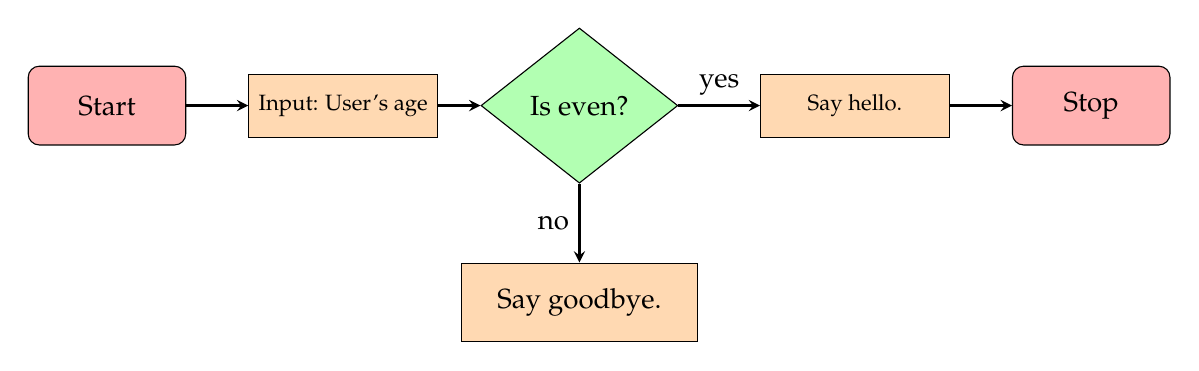
\begin{tikzpicture}[node distance=2cm]
                \node (start) [startstop] {Start};
                \node (in1) [process, right of=start, xshift=1cm, scale=0.8] {Input: User's age};
                \node (dec1) [decision, right of=in1, xshift=1cm] {Is even?};
                \node (proc1) [process, right of=dec1, xshift=1.5cm, scale=0.8] {Say hello.};
                \node (proc2) [process, below of=dec1, yshift=-0.5cm] {Say goodbye.};
                \node (end) [startstop, right of=proc1, xshift=1cm] {Stop};
                \draw [arrow] (start) -- (in1);
                \draw [arrow] (in1) -- (dec1);
                \draw [arrow] (dec1) -- node[anchor=south] {yes} (proc1);
                \draw [arrow] (dec1) -- node[anchor=east] {no} (proc2);
                \draw [arrow] (proc1) -- (end);
            \end{tikzpicture}
        \end{frame}

        \begin{frame}{Branching}
            \vspace{-3mm}
            \begin{columns}
                \column{0.5\textwidth}
                \inputminted[firstline=1, lastline=4, frame=single,framesep=2pt]{python3}{code-examples/branching.py}
                \inputminted[firstline=6, lastline=13, frame=single,framesep=2pt]{python3}{code-examples/branching.py}
                \column{0.5\textwidth}
                \inputminted[firstline=15, lastline=27, frame=single,framesep=2pt]{python3}{code-examples/branching.py}
            \end{columns}
            \begin{itemize}
                \item \texttt{<condition>} has a \textbf{\texttt{bool}} value (\texttt{True} or \texttt{False})
                \item Which expressions will be evaluated in which conditions?
            \end{itemize}
        \end{frame}

\end{document}